% auto-generated by v10_maketikz.m -- do not edit by hand
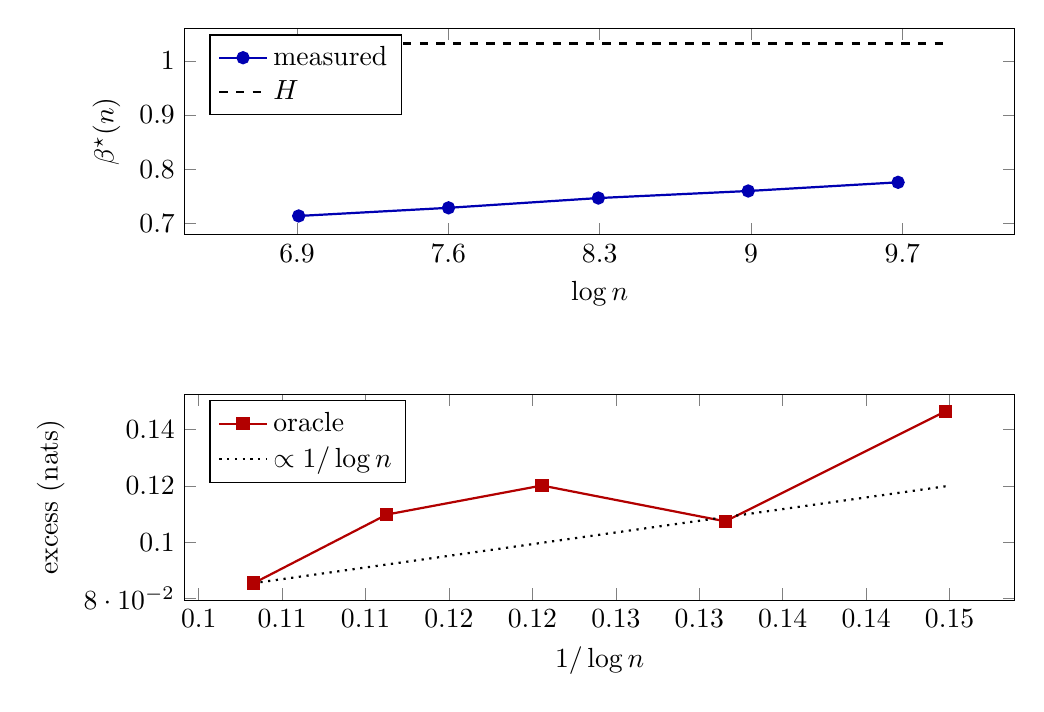
\begin{tikzpicture}
\begin{axis}[name=ax1,width=\linewidth,height=4.2cm,
  xlabel={$\log n$},ylabel={$\beta^\star(n)$},
  xtick={6.9,7.6,8.3,9,9.7},ymin=0.68,ymax=1.06,
  legend pos=north west,legend cell align=left,
  every axis plot/.append style={thick}]
\addplot[mark=*,blue!70!black] coordinates {(6.9078,0.714) (7.6009,0.729) (8.294,0.747) (8.9872,0.76) (9.6803,0.776) };
\addplot[black,dashed,no marks] coordinates {(6.7,1.0320)(9.9,1.0320)};
\legend{measured,$H$}
\end{axis}
\begin{axis}[name=ax2,at={(ax1.below south west)},anchor=above north west,yshift=-1.0cm,
  width=\linewidth,height=4.2cm,
  xlabel={$1/\log n$},ylabel={excess (nats)},
  legend pos=north west,legend cell align=left,
  every axis plot/.append style={thick}]
\addplot[mark=square*,red!70!black] coordinates {(0.14476,0.1464) (0.13156,0.1074) (0.12057,0.1201) (0.11127,0.1098) (0.1033,0.0855) };
\addplot[black,dotted,no marks] coordinates {(0.14476,0.11982) (0.13156,0.10889) (0.12057,0.099791) (0.11127,0.092094) (0.1033,0.0855) };
\legend{oracle,$\propto 1/\log n$}
\end{axis}
\end{tikzpicture}
